\chapter{Conclusion}

This chapter summarizes the accomplishments of the project over two semesters of research, design, and implementation. It also outlines the current limitations and potential directions for future development of the extension.

\section{Achieved Results}

We have developed an intelligent code assistance system tailored for web development, leveraging RAG to reduce hallucination and support integration of up-to-date information. The system is implemented as a Visual Studio Code extension named RAGGIN, Retrieval-Augmented Generation for Guided Intelligence in Next.js.

The project's source code is publicly available on GitHub under the MIT license\footnote{The MIT License — \url{https://opensource.org/license/mit}}, ensuring full transparency. The backend services\footnote{RAGGIN core service — \url{https://hub.docker.com/repository/docker/melukootto/raggin/general}} have been containerized and published on Docker Hub, while the extension frontend\footnote{RAGGIN Extension — \url{https://marketplace.visualstudio.com/items/?itemName=raggin.raggin}} is released on the Visual Studio Code Marketplace. Additionally, the processed Next.js documentation dataset used for retrieval has been made available on Kaggle\footnote{Next.js documentation dataset — \url{https://www.kaggle.com/datasets/jiyujizai/nextjs-documentation-for-raggin}}.

We have delivered a system that assists developers in integrating AI into their workflow, offering an open-source solution that grants the freedom to choose their preferred LLMs according to their system requirements. The system provides both deep configurability and flexibility while maintaining seamless integration within their familiar development environment.

\section{Limitations}

At present, the extension focuses exclusively on the Next.js framework, without support for the broader ecosystem of related technologies commonly used alongside it. While we have manually curated the documentation dataset, defined chunking strategies, and designed embedding pipelines specifically for Next.js, the system lacks the ability to automatically identify and process documentation from other frameworks. As a result, the extension cannot yet be scaled automatically to support additional technologies.

Currently, RAGGIN only offers configuration flexibility for the generator model (i.e., the LLM used for response generation). The embedding model for documentation remains fixed, with embeddings precomputed and bundled with the system. Moreover, the extension does not yet support local GPU-based embedding generation for user queries due to the complexities involved in GPU Docker setup and the additional size such support would impose on the container image.

In terms of retrieval performance, our core service exhibits low precision and recall at small Top-\(K\) values: Precision@1 is approximately 0.27, and Recall@1 is 0.05. Performance improves only at larger \(K\), indicating the retrieval system is currently not optimized for extracting highly relevant results with minimal context. This limitation negatively impacts downstream LLM performance, as more irrelevant documents are included in the prompt context.

The full system image occupies roughly 20GB on Docker (17.3GB for the core backend service and 2.7GB for the Milvus database), excluding the language model and Ollama runtime, which challenges our original lightweight deployment goals.

Finally, it is worth noting that RAGGIN is positioned as an open-source alternative to proprietary services like GitHub Copilot\footnote{GitHub Copilot — \url{https://github.com/features/copilot}}, which benefits from commercial-scale infrastructure and full integration with the Visual Studio Code ecosystem through its parent company, Microsoft.

\section{Future development directions}

To address the current limitations, we propose several concrete development directions aimed at improving scalability, configurability, performance, and portability of RAGGIN.

\paragraph*{Expanding framework support}

To broaden beyond Next.js, future work will focus on automating the identification and acquisition of documentation from other technologies, such as React\footnote{React — \url{https://reactjs.org}}, Vue\footnote{Vue — \url{https://vuejs.org}}, or TailwindCSS\footnote{Tailwind CSS — \url{https://tailwindcss.com}}. This may involve using sitemap parsing, structured data from \texttt{schema.org}\footnote{\texttt{schema.org} — \url{https://schema.org}}, or scraping via documentation RSS feeds. A modular preprocessing pipeline will also be developed to support customizable chunking and embedding per framework.

\paragraph*{Custom embedding model configuration}

Support for configurable embedding models will be introduced, allowing users to select their preferred models (e.g., BGE-M3, E5, or InstructorXL\footnote{InstructorXL — \url{https://huggingface.co/hkunlp/instructor-xl}}) during setup. Additionally, GPU-based embedding generation for user queries will be optionally enabled through a separate, GPU-enabled Docker image to prevent bloating the default container.

\paragraph*{Improving retrieval accuracy at low Top-\(K\)}

Include fine-tuning the embedding model on task-specific data, introducing learning-to-rank mechanisms for hybrid scoring, and employing lightweight rerankers such as MiniLM\footnote{MiniLM — \url{https://huggingface.co/nreimers/MiniLM-L6-H384-uncased}} or RankT5\footnote{RankT5 — \url{https://github.com/nyu-dl/dl4marco-2022}} to refine the top retrieved entries. These methods aim to increase the relevance of results with minimal context.

\paragraph*{Reducing system size}

To meet lightweight deployment goals, we plan to modularize services, separating the backend API, and embedding module into independently deployable containers. Further size reduction can be achieved through multi-stage Docker builds, minimal base images (e.g., Alpine\footnote{Alpine Linux — \url{https://alpinelinux.org}}).

\paragraph*{Ecosystem integration and tooling}

To enhance usability and ecosystem compatibility, future development will target integration with the Language Server Protocol (LSP)\footnote{Language Server Protocol (LSP) — \url{https://microsoft.github.io/language-server-protocol}}, enabling support beyond Visual Studio Code (e.g., WebStorm\footnote{WebStorm — \url{https://www.jetbrains.com/webstorm}}, Neovim\footnote{Neovim — \url{https://neovim.io}}).

These future directions aim to evolve RAGGIN into a robust, extensible, and developer-friendly tool that remains open, transparent, and adaptable to diverse workflows.

%% \section{Conclusion}
%
%Our work began in early September 2024, where we selected the problem to address based on our interests and familiarity with the domain. The problem definition phase focused on exploring how we can utilize LLMs to facilitate the development of a rapidly evolving framework while adhering to the latest guidelines. Concurrently, we conducted research on background knowledge. 
%
%We started by reading surveys on RAG systems \cite{zhao2024retrievalaugmentedgenerationaigeneratedcontent, gao2023ragllmsurvey} and delved into its core components:
%
%\begin{itemize}
%	\item \textbf{Retriever:} 
%	We began by determining how to represent data for semantic search. BGE-M3 \cite{chen2024bge} emerged as a suitable choice for English, supporting multiple search methods including sparse, dense, multi-vector, and hybrid search. To facilitate the search process efficiently, we studied KNN and its limitations, particularly regarding scalability in large databases. To address this, we adopted HNSW \cite{malkov2018hnsw}, which offers a balanced trade-off between accuracy and scalability for vector search.
%	
%	\item \textbf{Generator:}
%	For the generator, we built upon the Transformer architecture \cite{vaswani2017}, which serves as the foundation for LLMs, decoder-only transformer. We opted for Qwen \cite{bai2023qwen} as our model for generating text and code within the system.
%\end{itemize}
%
%Following this foundation, we investigated how augmentation could be integrated. We chose to augment the system during the inference stage, inspired by RALM \cite{ram2023incontext}. In essence, this stage occurs before the prompt is passed into the LLM, where we inject documentation content into the prompt via string concatenation. 
%
%The augmentation source consists of structured and unstructured data derived from the Next.js documentation. The structured data pertains to the organization of the documentation, while the unstructured data includes code samples. To manage this data effectively, we adopted the KnowledgeGPT framework \cite{wang2023knowledgpt}, organizing the data into a knowledge base while supporting semantic search for unstructured content. For the augmentation process, we applied adaptive methods to determine when external information is necessary to generate accurate answers, utilizing reflection tokens as implemented in SELF-RAG \cite{asai2023selfrag}.
%
%Based on our supervisors' suggestions, we decided to deliver our solution as a VSCode extension. To inform this decision, we analyzed related tools by examining their retrieval mechanisms, code generation capabilities, and integration within the development process. After a thorough comparison, we decided that our solution would run entirely locally on the user’s machine, focusing on performance with limited resources. This approach allows us to evaluate our solution against existing cloud-based, paid alternatives like GitHub Copilot\footnote{GitHub Copilot - \url{https://copilot.github.com/}}.
%
%Subsequently, we finalized our approach and designed a high-level architecture (Figure~\ref{fig:RAG-architecture}). For the database, we chose Milvus \cite{wang2021milvus} due to its open-source nature and comprehensive SDK support.
%
%We proceeded with the initial implementation of the system, starting with data preparation. This involved identifying the data source, extracting content from the official Next.js GitHub repository, and implementing preprocessing scripts to clean and process markdown files. We then embedded the data and stored it in the database. As a preliminary milestone, we developed a demonstration script capable of taking an input string and retrieving relevant documents from the database. This phase did not yet include prompt engineering or advanced retrieval mechanisms.
%
%We then outlined our evaluation strategy, which focuses on two key components:
%\begin{enumerate}
%	\item Evaluating the RAG components: retriever and generator performance.
%	\item Testing the VSCode extension as a software product.
%\end{enumerate}
%
%Report writing began in October 2024, based on slides prepared for weekly supervisor meetings. We continued to write and refine the report following feedback and guidance from our supervisors.


% \begin{figure}[H]
%     \centering
%     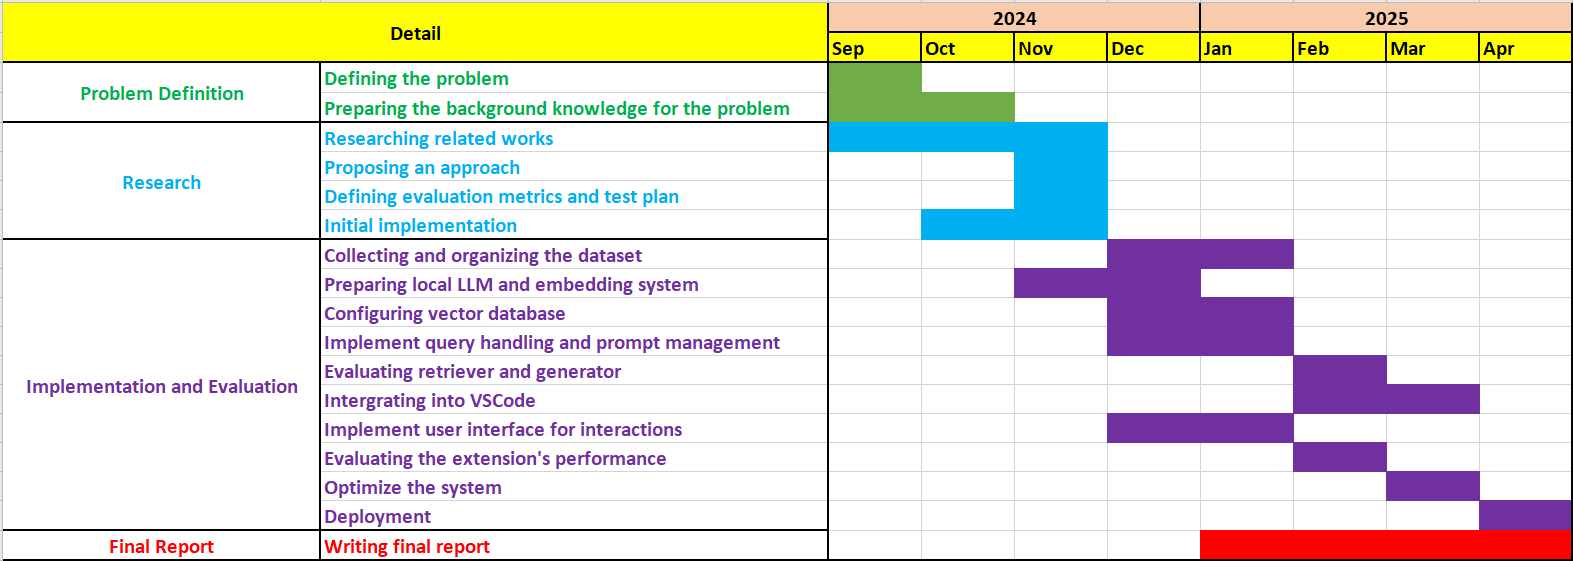
\includegraphics[width=\linewidth]{Images/Conclusion/future_plan_gantt.png}
%     \vspace{0.35cm}
%     \caption{Future plan}
%     \label{fig:future-plan}
% \end{figure}

% \begin{figure}[tbp]
%     \begin{center}
    
%     \begin{ganttchart}[y unit title=0.4cm,
%     y unit chart=0.5cm,
%     x unit=0.7cm,
%     vgrid,hgrid, 
%     % bar/.append style={fill=blue!40, align=left, text width=4cm, text left shift=0.2cm}, % Aligns text left
%     % bar height=0.6,
%     title label anchor/.style={below=-1.6ex},
%     title left shift=.05,
%     title right shift=-.05,
%     title height=1,
%     progress label text={},
%     bar height=0.7,
%     group right shift=0,
%     group top shift=.6,
%     group height=.3]{1}{16}
%     %labels
%     \gantttitle{2024}{8}
%     \gantttitle{2025}{8} \\
%     \gantttitle{Sep}{2} 
%     \gantttitle{Oct}{2} 
%     \gantttitle{Nov}{2} 
%     \gantttitle{Dec}{2} 
%     \gantttitle{Jan}{2} 
%     \gantttitle{Feb}{2} 
%     \gantttitle{Mar}{2} 
%     \gantttitle{Apr}{2} \\
%     %tasks
%     \ganttgroup[progress=100]{Problem Definition}{1}{6} \\
    
%     \ganttbar[progress=100]{Defining the problem}{1}{2}\\
%     \ganttbar[progress=100]{Preparing the background knowledge for the problem}{1}{4}\\

%     \ganttgroup[progress=100]{Research}{1}{9} \\
    
%     \ganttbar[progress=100]{Researching related works}{1}{9}\\
%     \ganttbar[progress=100]{Proposing an approach}{1}{4}\\
%     \ganttbar[progress=100]{Defining evaluation metrics and test plan}{1}{4}\\
    
%     % \ganttbar{first task}{1}{2} \\
%     % \ganttbar{task 2}{3}{8} \\
%     % \ganttbar{task 3}{9}{10} \\
%     % \ganttbar{task 4}{11}{15} \\
%     % \ganttbar[progress=33]{task 5}{20}{22} \\
%     % \ganttbar{task 6}{18}{19} \\
%     % \ganttbar{task 7}{16}{18} \\
%     % \ganttbar[progress=0]{task 8}{21}{24}
    
%     %relations 
%     % \ganttlink{elem0}{elem1} 
%     % \ganttlink{elem0}{elem3} 
%     % \ganttlink{elem1}{elem2} 
%     % \ganttlink{elem3}{elem4} 
%     % \ganttlink{elem1}{elem5} 
%     % \ganttlink{elem3}{elem5} 
%     % \ganttlink{elem2}{elem6} 
%     % \ganttlink{elem3}{elem6} 
%     % \ganttlink{elem5}{elem7} 
%     \end{ganttchart}
%     \end{center}
%     \caption{Gantt Chart}

% \end{figure}

% \begin{ganttchart}{1}{12}
%   \gantttitle{2011}{12} \\
%   \gantttitlelist{1,...,12}{1} \\
%   \ganttgroup{Group 1}{1}{7} \\
%   \ganttbar{Task 1}{1}{2} \\
%   \ganttlinkedbar{Task 2}{3}{7} \ganttnewline
%   \ganttmilestone{Milestone}{7} \ganttnewline
%   \ganttbar{Final Task}{8}{12}
%   \ganttlink{elem2}{elem3}
%   \ganttlink{elem3}{elem4}
% \end{ganttchart}



% \section{Upcoming works: January 2025 and beyond}
%
%
%\begin{enumerate}
%	\item \textbf{Preparing local LLM and embedding system (November 2024 -- January 2025):}
%	Setup and configure the local LLM and embedding system to handle efficient information retrieval.
%	
%	\item \textbf{Collecting and organizing the dataset (December 2024 -- February 2025):}
%	Data collection and preprocessing efforts will focus on organizing high-quality and relevant datasets.
%	
%	\item \textbf{Configuring vector database (December 2024 -- February 2025):}
%	Establish the vector database to efficiently store and retrieve embeddings for core functionalities.
%	
%	\item \textbf{Implementing query handling and prompt management (December 2024 -- February 2025):}
%	Mechanisms for managing user queries and prompt workflows will be implemented for smooth operations.
%	
%	\item \textbf{Evaluating retriever and generator (February -- March 2025):}
%	Assessment of retrieval and generation components for accuracy, efficiency, and robustness.
%	
%	\item \textbf{Integrating into VSCode (February -- April 2025):}
%	The system will be integrated into the VSCode environment as an extension to improve developer accessibility.
%	
%	\item \textbf{Implementing user interface for interactions (January -- April 2025):}
%	Develop an intuitive and interactive user interface to ensure seamless user experience.
%	
%	\item \textbf{Evaluating the extension's performance (March -- April 2025):}
%	Performance testing of the VSCode extension will focus on usability, responsiveness, and reliability.
%	
%	\item \textbf{Optimizing the system (March -- May 2025):}
%	Optimize the system to enhance efficiency, accuracy, and overall performance.
%	
%	\item \textbf{Deployment (April -- May 2025):}
%	Fully develop, test, and deploy the optimized system for production use.
%	
%	\item \textbf{Continue writing report (December 2024 -- May 2025):}
%	Prepare the final report summarizing the problem definition, research, implementation, evaluation, and findings.
%\end{enumerate}
%
%% \hspace{-4cm}
%\begin{figure}[tbp]
%	% \begin{center}
%		\hspace*{-2cm} 
%		\begin{ganttchart}[
%			y unit title=0.4cm,
%			y unit chart=0.6cm,
%			x unit=0.6cm,
%			vgrid,
%			hgrid,
%			title label anchor/.style={below=-1.6ex},
%			title left shift=.05,
%			title right shift=-.05,
%			title height=1,
%			progress label text={},
%			bar height=0.6,
%			group right shift=0,
%			group top shift=.6,
%			group height=.3
%			]{1}{18}
%			
%			% Year and Month Titles
%			\gantttitle{2024}{8}
%			\gantttitle{2025}{10} \\
%			\gantttitle{Sep}{2}
%			\gantttitle{Oct}{2}
%			\gantttitle{Nov}{2}
%			\gantttitle{Dec}{2}
%			\gantttitle{Jan}{2}
%			\gantttitle{Feb}{2}
%			\gantttitle{Mar}{2}
%			\gantttitle{Apr}{2} 
%			\gantttitle{May}{2} \\
%			
%			% Problem Definition Group
%			\ganttgroup[/pgfgantt/group/.style={},inline=false]{Problem Definition}{1}{7} \\
%			\ganttbar[bar/.append style={fill={dkgreen}}]{Defining the problem}{1}{3} \\
%			\ganttbar[bar/.append style={fill={dkgreen}}]{Preparing background knowledge}{1}{5} \\
%			
%			% Research Group
%			\ganttgroup[/pgfgantt/group/.style={},inline=false]{Research}{1}{7} \\
%			\ganttbar[bar/.append style={fill=cyan}]{Researching related works and tools}{1}{6} \\
%			\ganttbar[bar/.append style={fill=cyan}]{Proposing an approach}{4}{6} \\
%			\ganttbar[bar/.append style={fill=cyan}]{Defining evaluation metrics and test plan}{5}{7} \\
%			\ganttbar[bar/.append style={fill=cyan}]{Initial implementation}{4}{7} \\
%			\ganttbar[bar/.append style={fill=cyan}]{Writing report}{3}{7} \\
%			% Implementation and Evaluation Group
%			\ganttgroup[/pgfgantt/group/.style={},inline=false]{Implementation and evaluation}{5}{18} \\
%			\ganttbar[bar/.append style={fill={codepurple}}]{Preparing local LLM and embedding system}{5}{9} \\
%			\ganttbar[bar/.append style={fill={codepurple}}]{Collecting and organizing dataset}{7}{11} \\
%			\ganttbar[bar/.append style={fill={codepurple}}]{Configuring vector database}{7}{11} \\
%			\ganttbar[bar/.append style={fill={codepurple}}]{Implementing query handling and prompt management}{9}{13} \\
%			\ganttbar[bar/.append style={fill={codepurple}}]{Evaluating retriever and generator}{11}{13} \\
%			\ganttbar[bar/.append style={fill={codepurple}}]{Integrating into VSCode}{11}{15} \\
%			\ganttbar[bar/.append style={fill={codepurple}}]{Implementing user interface for interactions}{7}{13} \\
%			% \ganttbar[progress=10]{Implement user interface for interactions}{13}{14} \\
%			\ganttbar[bar/.append style={fill={codepurple}}]{Evaluating the extension's performance}{13}{16} \\
%			\ganttbar[bar/.append style={fill={codepurple}}]{Optimizing the system}{14}{17} \\
%			\ganttbar[bar/.append style={fill={codepurple}}]{Deployment}{15}{17} \\
%			
%			% Final Report Group
%			\ganttgroup[/pgfgantt/group/.style={},inline=false]{Final report}{9}{18} \\
%			\ganttbar[bar/.append style={fill=red}]{Continue writing report}{9}{17} \\
%			
%		\end{ganttchart}
%		% \end{center}
%	\vspace{2mm}
%	\caption{Future works.}
%\end{figure}
%  